\documentclass{beamer}
\usetheme{default}
\setbeamertemplate{navigation symbols}{}
%	
\usepackage{subfig}
\usepackage{epstopdf}
\usepackage{amsmath, amsthm, amssymb}
\usepackage{float}
\usepackage{rotating}
\usepackage{graphicx}
\usepackage{longtable}
\usepackage{xcolor}
\usepackage{bm}
\usepackage{tikz}
\usetikzlibrary{shapes}
\newcommand{\EE}{\mathbb E}
\newcommand{\var}{\mathrm{var}}
\newcommand{\cov}{\mathrm{cov}}
\newtheorem{acknowledgement}[theorem]{Acknowledgement}
\newtheorem{algorithm}[theorem]{Algorithm}
\newtheorem{assumption}{Assumption}
\newtheorem{axiom}{Axiom}
\newtheorem{case}[theorem]{Case}
\newtheorem{claim}[theorem]{Claim}
\newtheorem{conclusion}[theorem]{Conclusion}
\newtheorem{condition}[theorem]{Condition}
\newtheorem{conjecture}{Conjecture}
\newtheorem{criterion}[theorem]{Criterion}
\newtheorem{proposition}{Proposition}
\newtheorem{summary}[theorem]{Summary}
\newtheorem{exercise}{Exercise}
\newtheorem{notation}{Notation}
\newtheorem{remark}{Remark}
%\graphicspath{{graphs//}}

\title {BEGS: Quantitative Results}

\date{September 2013}
% \today will show current date.
% Alternatively, you can specify a date.
%
\begin{document}
%
\begin{frame}
\titlepage

\end{frame}


\begin{frame}
\frametitle{Numerical exercise}
 
Solve a $N=5$ agent economy with realistic level and movements in wage dispersion across booms and recessions

\begin{itemize}
 \item Long run dynamics: Study settings that differ in covariance of interest rates and output
 \item Transient dynamics: Study outcomes in recessions that are accompanied by higher inequality
\end{itemize}

Aggregate shocks affect,
\begin{enumerate}
\item Wages: \[\log \theta_i=\epsilon [1+(.9-i)m]\]
 \item Payoffs: \[P=1+\chi \epsilon \]
\end{enumerate}

\end{frame}

\begin{frame}
\frametitle{Calibration}

\begin{table}[htp]
\small
\begin{tabular}{|l|c|p{4cm}|}
\hline
Parameter & Value & Description   \\ \hline
$\{\bar{\theta}_i\} $ & \{1 ,  1.4,  2.1,  3.24,  4.9\} & Wages dispersion for \{10,25,50,25,90\} percentiles   \\
$\psi$ & 0.53 & Average Frisch elasticity of labor supply of 1 \\
$\beta$ & 0.98  &Average (annual) risk free interest rate of 2\%   \\
$m$ &$\frac{1.5}{.8}$& Changes in dispersion \\
$\sigma_e$ & 0.03 & Business cycle fluctuations in wages\\
$g$ & .13 \%&Average pre-transfer expenditure- output ratio of 12 \% \\\hline

\end{tabular}
\caption{Benchmark calibration}
\label{tab:Parameters}
\end{table}

The Pareto weights and initial distribution of wealth is chosen to match an average tax rate of $20\%$ and debt to gdp ratio of $60\%$ and transfers to gdp ratio of 10\%. 

\end{frame}


\begin{frame}
\frametitle{Long run}
 {
  \begin{figure}
    \centering
    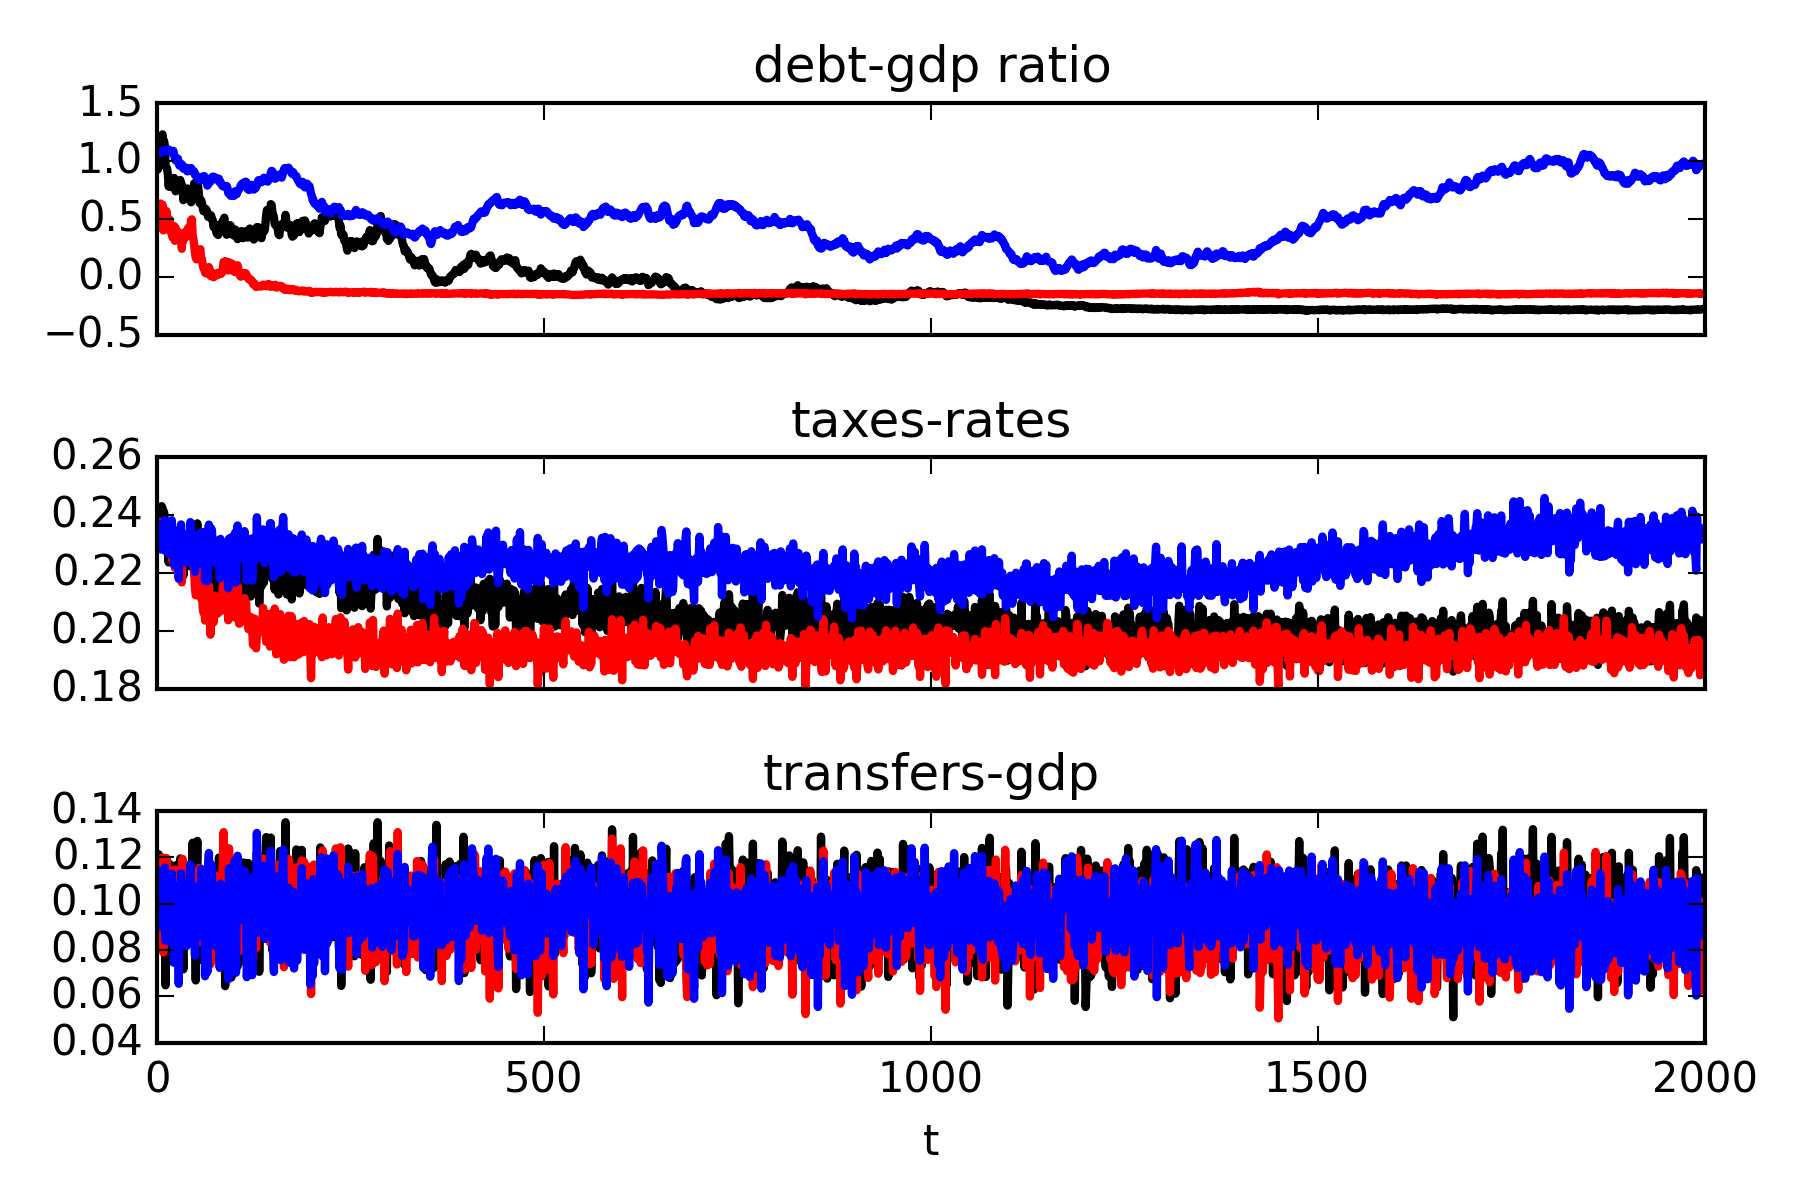
\includegraphics[width = 0.9\textwidth]{plots/long_simulation_debt.png}
    \caption{The red, black and blue lines plot simulations for a common sequence of shocks for values of $\chi=-1.5,0,1.5$ respectively}
  \end{figure}

}

\end{frame}


\begin{frame}
\frametitle{Long run: Speed of convergence}
 {
  \begin{figure}
    \centering
    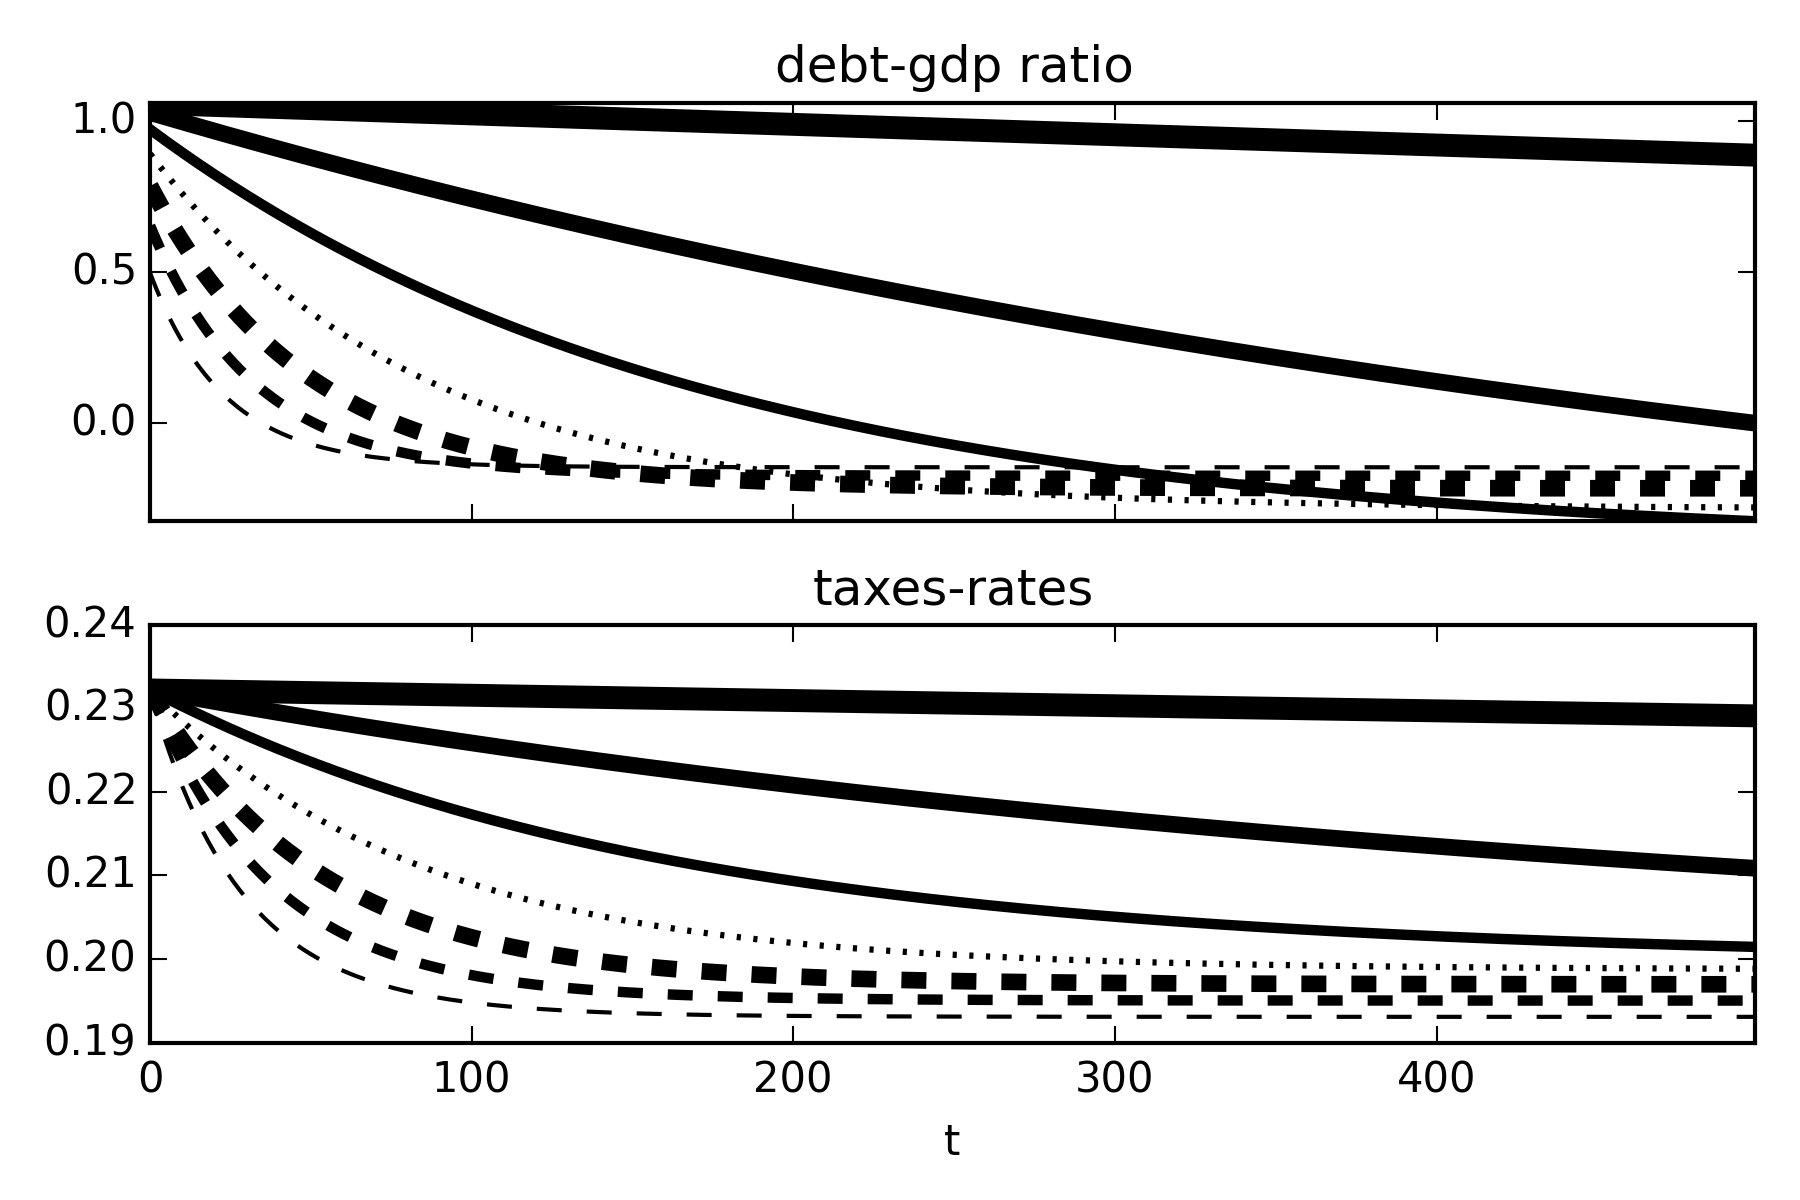
\includegraphics[width = 0.9\textwidth]{plots/speed_of_convergence.png}
    \caption{The plot shows conditional mean paths for different values of $\chi$. The red (blue) lines have $\chi<0$ ($\chi>0$). The thicker lines represent larger values.}
  \end{figure}

}

\end{frame}



\begin{frame}
\frametitle{Short run}
Lets denote consecutive period of negative (positive) one s.d $\epsilon$ shocks a ``recession'' (boom)

\begin{itemize}
\item Simulate a recession that is followed by no further shocks
 
 \item Decompose responses into TFP component and inequality component:
  
 \vspace{3mm}
\centering  \textbf{Baseline:} $\log \theta_i=\epsilon [1+(.9-i)m]$
 \vspace{3mm}
 \begin{itemize}
  \item Only TFP: \[\log \theta_i=\epsilon\]
  \item Only Ineq: \[\log \theta_i=\epsilon [(.9-i)m]\]
\end{itemize}

\end{itemize}
 
\end{frame}


\begin{frame}
\frametitle{Recessions with higher inequality: Risk free bond,$\chi=0$}
{
  \begin{figure}
    \centering
    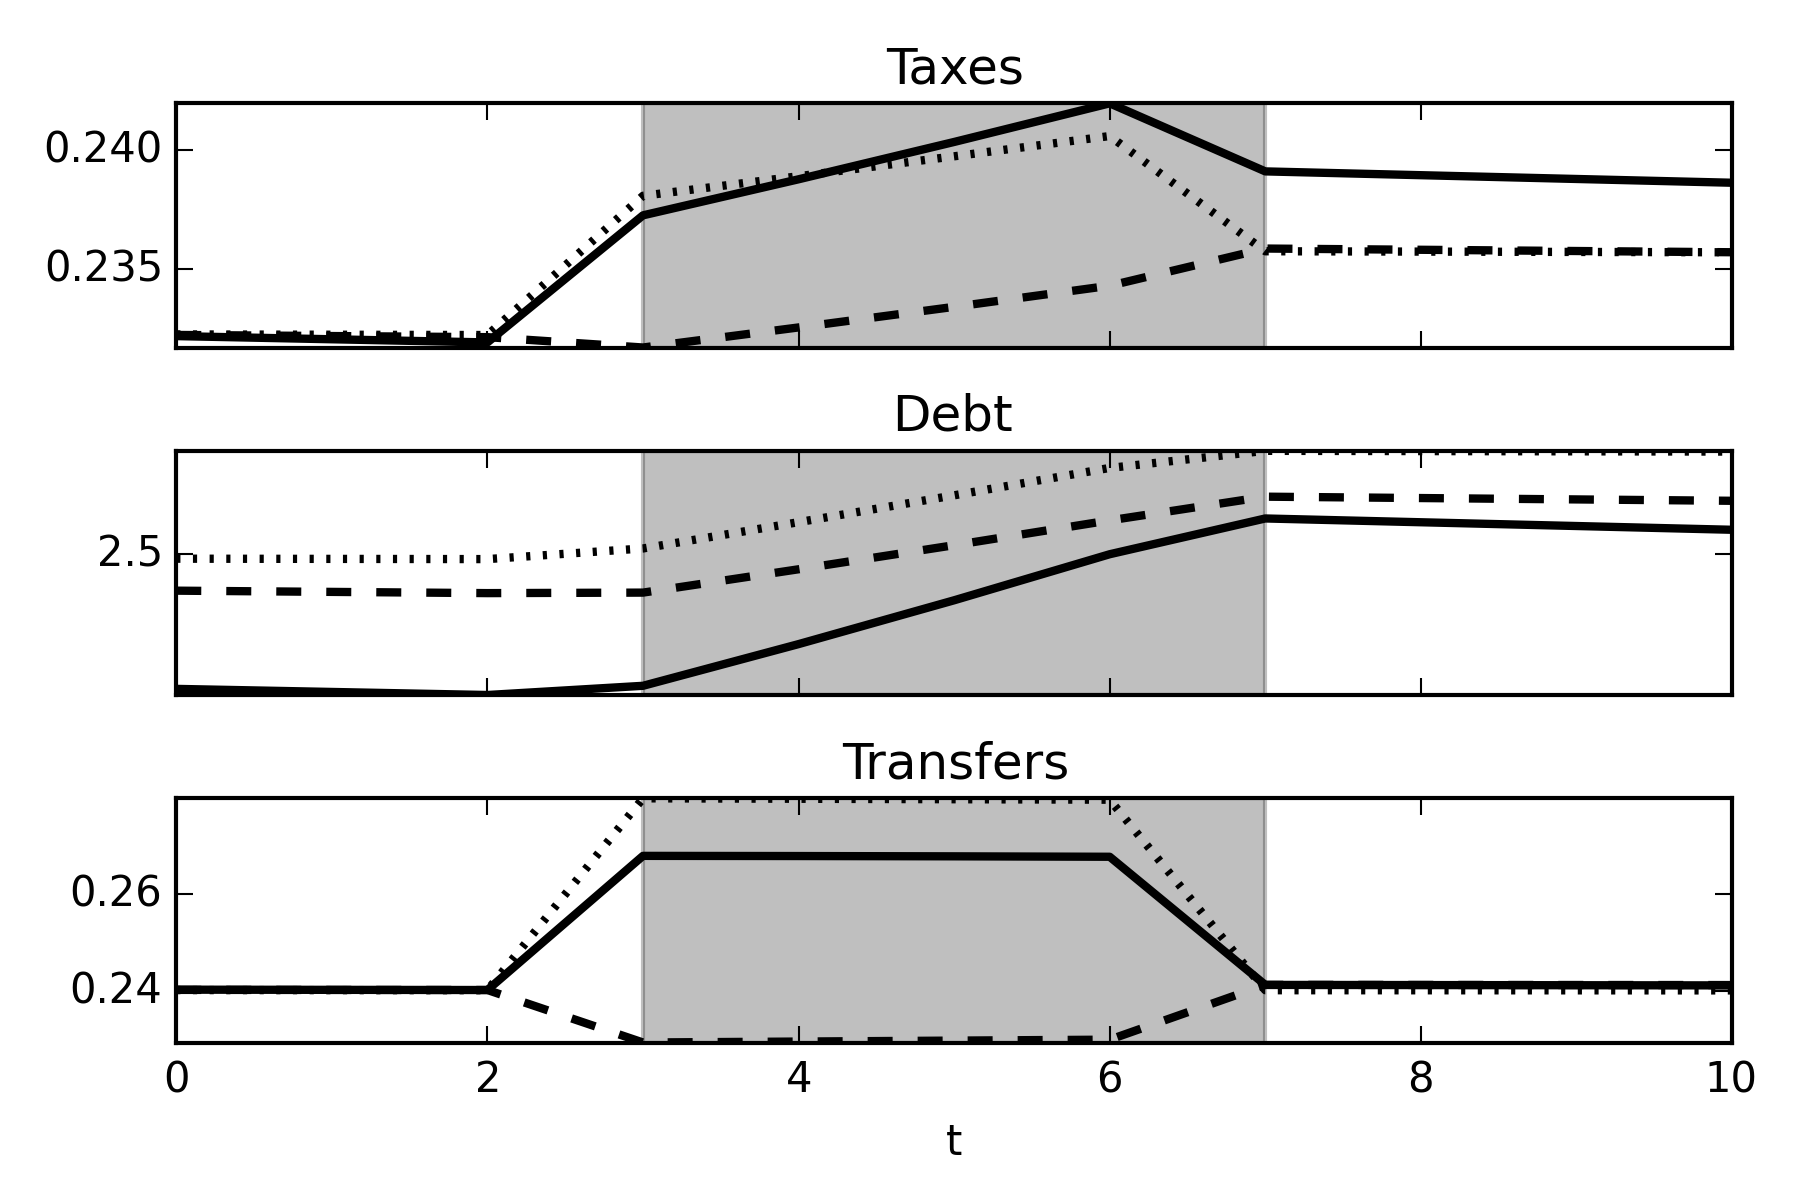
\includegraphics[width = 0.9\textwidth]{plots/irf_zero_chi_shocks.png}
    \caption{The bold line is the total response. The dashed (dotted) line reflects the only TFP (inequality) effect. The shaded region is the recession}
  \end{figure}

} 
\end{frame}

\begin{frame}
\frametitle{Recessions with higher inequality: Procyclical returns,$\chi>0$}
{
  \begin{figure}
    \centering
    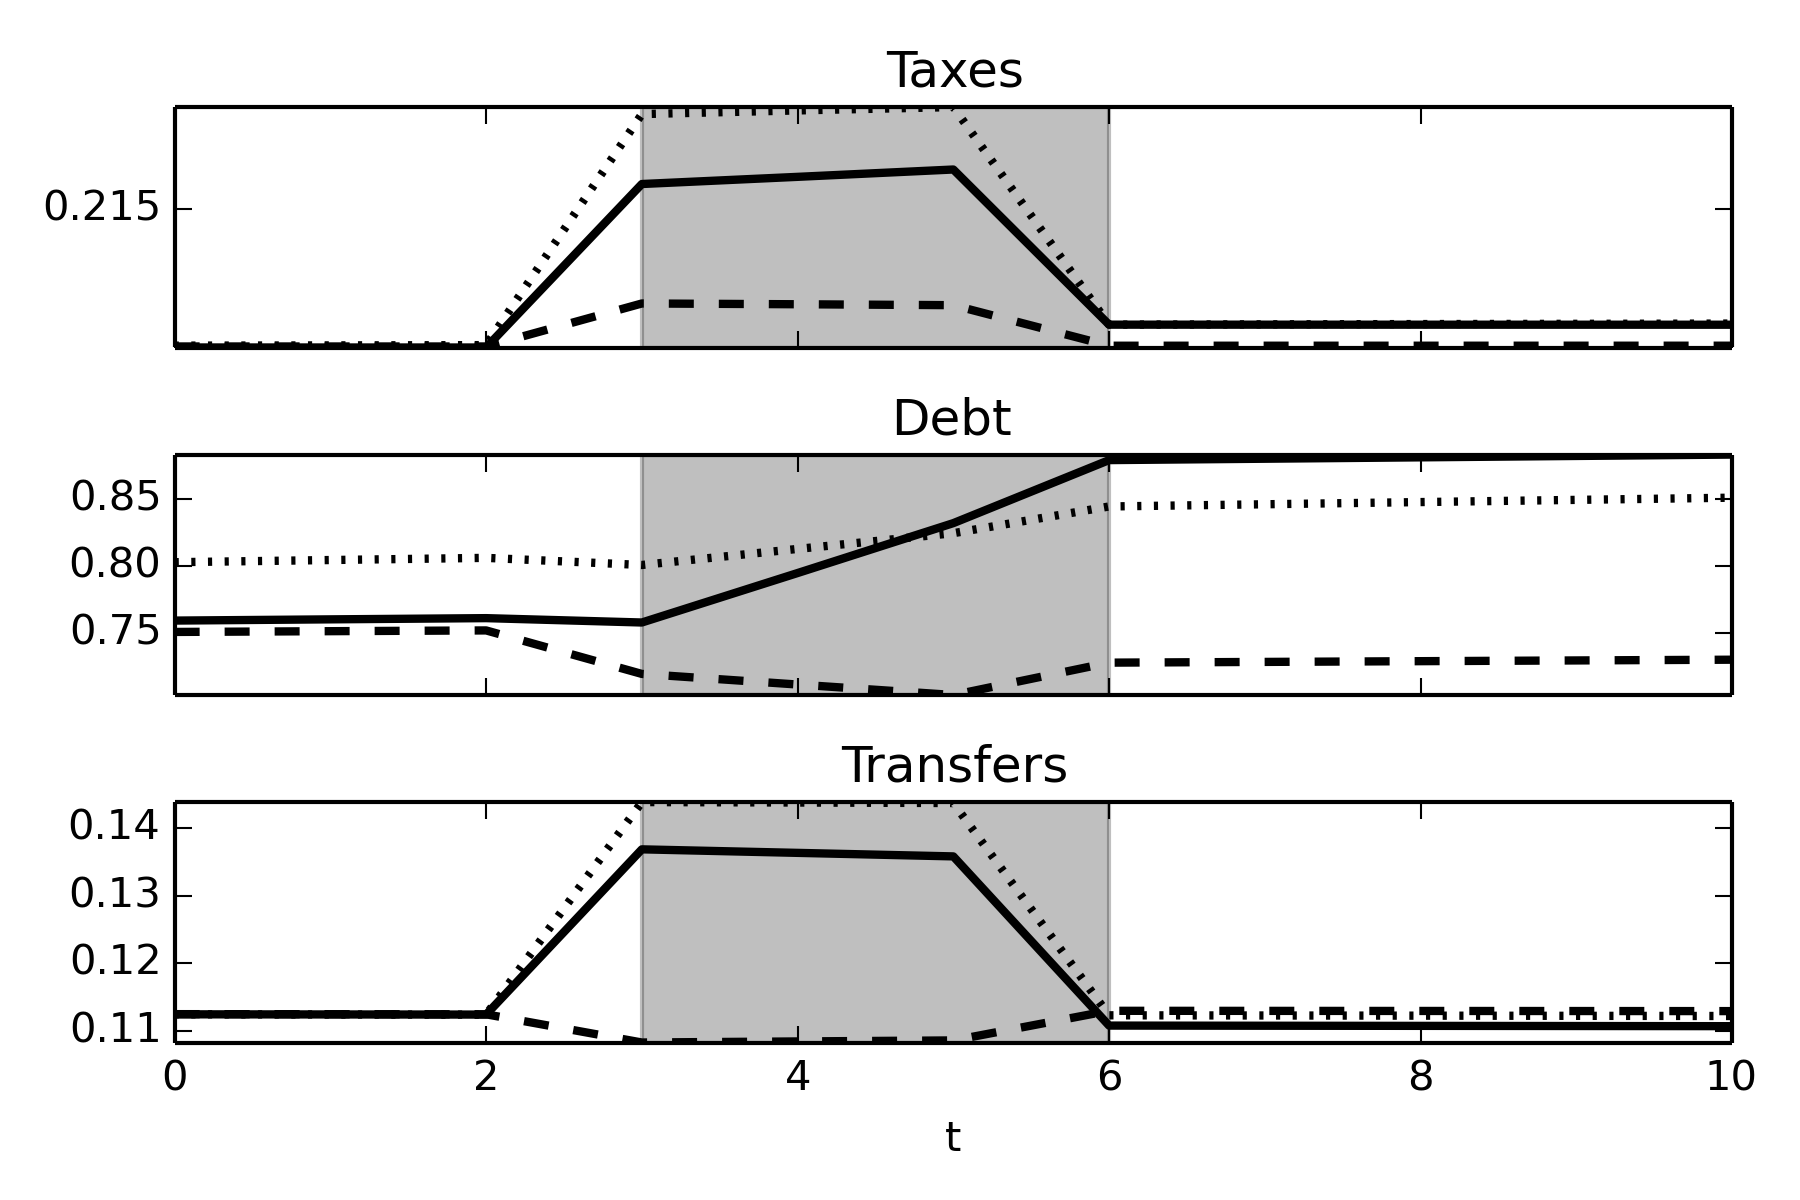
\includegraphics[width = 0.9\textwidth]{plots/irf_pos_chi_shocks.png}
    \caption{The bold line is the total response. The dashed (dotted) line reflects the only TFP (inequality) effect. The shaded region is the recession}
  \end{figure}

} 
\end{frame}


\begin{frame}
\frametitle{Recessions with higher inequality: Counter-cyclical returns,$\chi<0$}
{
  \begin{figure}
    \centering
    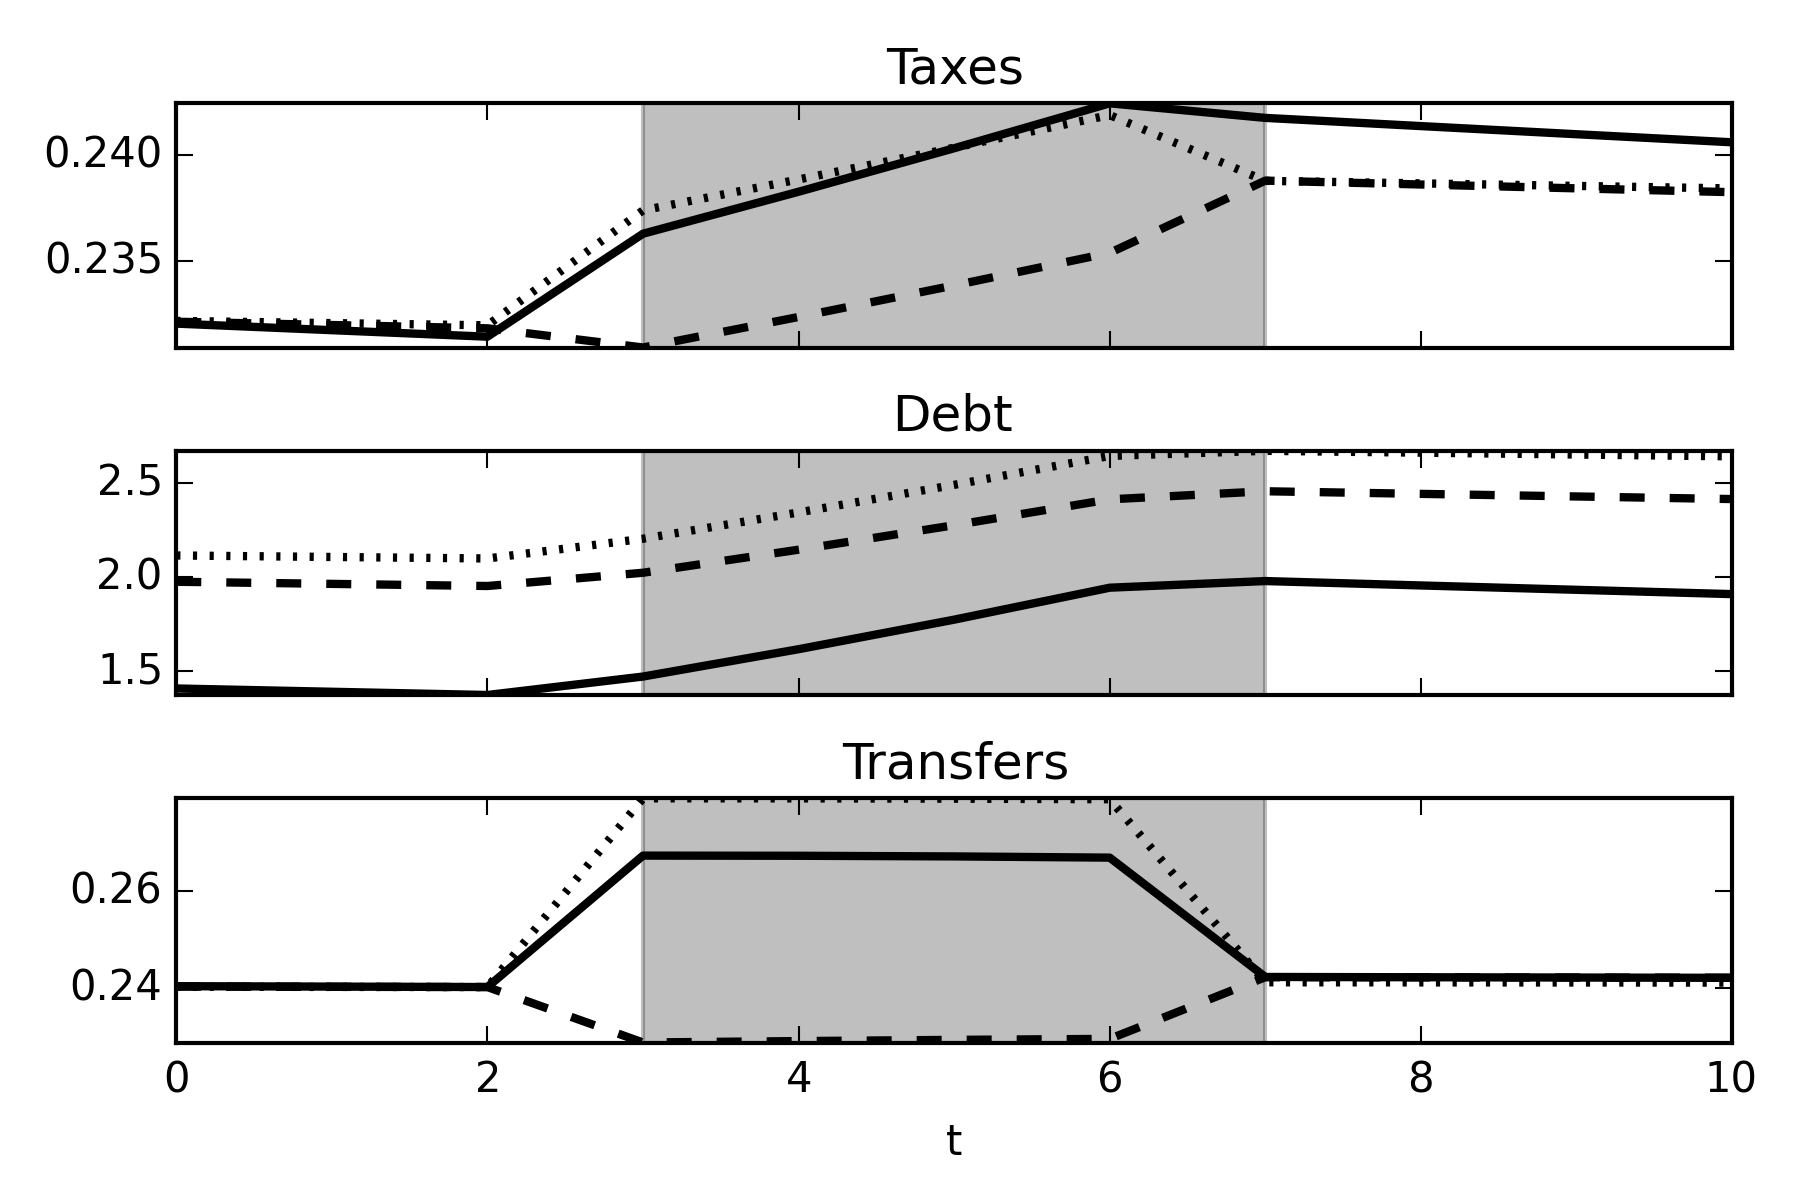
\includegraphics[width = 0.9\textwidth]{plots/irf_negative_chi_shocks.png}
    \caption{The bold line is the total response. The dashed (dotted) line reflects the only TFP (inequality) effect. The shaded region is the recession}
  \end{figure}

} 
\end{frame}

\begin{frame}
\frametitle{Redistribution in recessions}
\begin{itemize}
 \item TFP : Relative inequality is unchanged and planner redistributes by lowering tax-rates on impact.
 \item Only Ineq : Earnings gap increases by factor $m$. The planner mainly redistributes mainly through higher transfers and taxes.
 \item TFP + Ineq: For both tax rates and transfers are higher.
\end{itemize}
In all cases the burden is spread over time by lower future transfers and higher tax rates. 
\end{frame}


 \end{document}